\documentclass[12pt]{article}

\usepackage[brazilian]{babel}
\usepackage[utf8]{inputenc}
\usepackage[T1]{fontenc}
\usepackage{graphicx}
\everymath{\displaystyle}
\usepackage{amssymb}



\begin{document}
\date{}
\title{1ª PROVA DE CÁLCULO}
\author{Prof. Renato Vidal da Silva Martins}
\maketitle

\part{Enunciados}
\begin{enumerate}
	\item Calcule os limites abaixo, explicando seu raciocínio:
	\begin{enumerate}
		\item $ \lim\limits_{x \rightarrow 4} \frac{x^2-16}{\sqrt{x}-2} $
		\item $ \lim\limits_{x \rightarrow \infty} \frac{x^5+x^3+1}{-x^4+x^2+3} $
		\item $ \lim\limits_{x \rightarrow 2} \frac{\sin(x-2)}{x^2-6x+8} $
	\end{enumerate}
	\item Um cone de $1 cm$ de raio, $2 cm$ de altura está cheio de água. Fazendo um furo no bico, começa a vazar a uma taxa de $\pi/4$ $cm^3/s$. Calcule a taxa de variação do nível de água no instante em que 7/8 do volume já vazou.
	\item Calcule a derivada $dy/dx$, onde:
	\begin{enumerate}
		\item $ y = \frac{x^5+x^3+1}{-x^4+x^2+3} $
		\item $ y = \tan(\sqrt{x^3+1}) $
		\item $ y = x^9 \cos^5(x) $
	\end{enumerate}
	
	\item Equacione a reta tangente á curva abaixo no ponto $(0,1)$:
	\begin{center}
		$ \left( x + y \right)^4 -7x^2 + y = 2  $\\
	\end{center}
\end{enumerate}

\newpage
\part{Resolução}
\begin{enumerate}
	\item Calcule os limites abaixo, explicando seu raciocínio:
	\begin{enumerate}
		\item $ \lim\limits_{x \rightarrow 4} \frac{x^2-16}{\sqrt{x}-2} $\\
		\\Começamos desenvolvendo os termos para sair da indeterminação $0/0$:
		\begin{center}
			$ \lim\limits_{x \rightarrow 4} \frac{x^2-16}{\sqrt{x}-2} . \frac{\sqrt{x}+2}{\sqrt{x}+2} $\\
			$ \lim\limits_{x \rightarrow 4} \frac{(x-4)(x+4)(\sqrt{x}+2)}{x-4} $\\
			$ \lim\limits_{x \rightarrow 4} (x+4)(\sqrt{x}+2) = 32 $\\
		\end{center}
		Logo:
		\begin{center}
			$ \lim\limits_{x \rightarrow 4} \frac{x^2-16}{\sqrt{x}-2} = 32$
		\end{center}
		
		\item $ \lim\limits_{x \rightarrow \infty} \frac{x^5+x^3+1}{-x^4+x^2+3} $
		\\
		\\Basta colocar $x^4$ em evidência, temos:
		\begin{center}
			$ \lim\limits_{x \rightarrow \infty} \frac{x^4 \left( x+ \frac{1}{x}+\frac{1}{x^4} \right) }{x^4 \left( -1+ \frac{1}{x^2} + \frac{3}{x^4} \right) } $\\
			$ \lim\limits_{x \rightarrow \infty} \frac{\left( x+ \frac{1}{x}+\frac{1}{x^4} \right) }{\left( -1+ \frac{1}{x^2} + \frac{3}{x^4} \right) } $
		\end{center}
		Como os termos com $x$ no denominador tendem a zero quando $x \rightarrow \infty$:
		\begin{center}
			$ \lim\limits_{x \rightarrow \infty} \frac{\left( x+ 0+0 \right) }{\left( -1+ 0 + 0 \right) } = -x = -\infty $
		\end{center}
		Logo:
		\begin{center}
			$ \lim\limits_{x \rightarrow \infty} \frac{x^5+x^3+1}{-x^4+x^2+3} = -\infty$
		\end{center}
		
		\item $ \lim\limits_{x \rightarrow 2} \frac{\sin(x-2)}{x^2-6x+8} $\\
		\\Vamos desenvolver a equação de segundo grau:
		\begin{center}
			$ \lim\limits_{x \rightarrow 2} \frac{\sin(x-2)}{(x-2)(x-4)} $
		\end{center}
		Pelo limite do seno:
		\begin{center}
			$ \lim\limits_{x \rightarrow 2} \frac{1}{x-4} = -\frac{1}{2} $
		\end{center}
		Seguindo:
		\begin{center}
			$ \lim\limits_{x \rightarrow 2} \frac{\sin(x-2)}{(x-2)(x-4)} = -\frac{1}{2} $
		\end{center}
		
	\end{enumerate}
	\item Um cone de $1 cm$ de raio, $2 cm$ de altura está cheio de água. Fazendo um furo no bico, começa a vazar a uma taxa de $\pi/4$ $cm^3/s$. Calcule a taxa de variação do nível de água no instante em que 7/8 do volume já vazou.\\
	\\
	O exercício pede a taxa de variação do nível da água no instante em que restam 1/8 do conteúdo original, para tanto é preciso escrever a função que fornece a altura em função do volume dado.\\
	Observando a formula do volume e tendo em mente semelhança de triângulos podemos notar que quando a altura é reduzida a uma porcentagem $x$ o volume todo é reduzido a uma porcentagem $x^3$ do original. Ou seja:\\
	
	\begin{center}
		$ Volume_{atual} = \left( \frac{Altura_{atual}}{Altura_{inicial}} \right)^3 \times Volume_{inicial} $\\
		$ Volume_{atual} = Volume_{inicial} - \frac{\pi t}{4} = \frac{8\pi - 3\pi t}{12}$\\
		$ Altura_{atual} = Altura_{inicial} \sqrt[3]{\frac{Volume_{atual} }{Volume_{inicial} } }$\\
		
		$ h(V) = h_{0} \sqrt[3]{\frac{V}{V_{0} } } = 2\sqrt[3]{\frac{3V}{2\pi}}   $\\
		
		$ h(t) = 2 \sqrt[3]{\frac{8 - 3t}{8} }$\\
	\end{center}
	
	Para calcular o volume inicial basta tomar a fórmula:
	
	\begin{center}
		$\frac{\pi r^2 h}{3} = \frac{\pi 1^2.2}{3} = \frac{2\pi}{3}$
	\end{center}
	
	O volume que queremos localizar é:
	
	\begin{center}
		$\frac{1}{8}.\frac{2\pi}{3} = \frac{\pi}{12}$
	\end{center}
	
	A taxa de variação da altura em um momento é a sua derivada, então:
	
	\begin{center}
		$ \left[ 2 \sqrt[3]{\frac{8 - 3t}{8}} \right] ' = -\frac{1}{4} \left( \frac{8}{8-3t}\right) ^{\frac{2}{3}} $\\
	\end{center}
	
	Vamos descobrir o tempo igualando na equação do volume em função do tempo:
	
	\begin{center}
		$ \frac{\pi}{12} = \frac{8\pi - 3\pi t}{12}$\\
		$ t = \frac{7}{3}$\\
	\end{center}
	
	Substituindo no ponto teremos:
	
	\begin{center}
		$ -\frac{1}{4} \left( \frac{8}{8-3 \times \frac{7}{3}}\right) ^{\frac{2}{3}} = -1$\\
	\end{center}
	
	Então a taxa de variação no instante requerido é de $-1 cm/s$.
	
	\begin{center}
		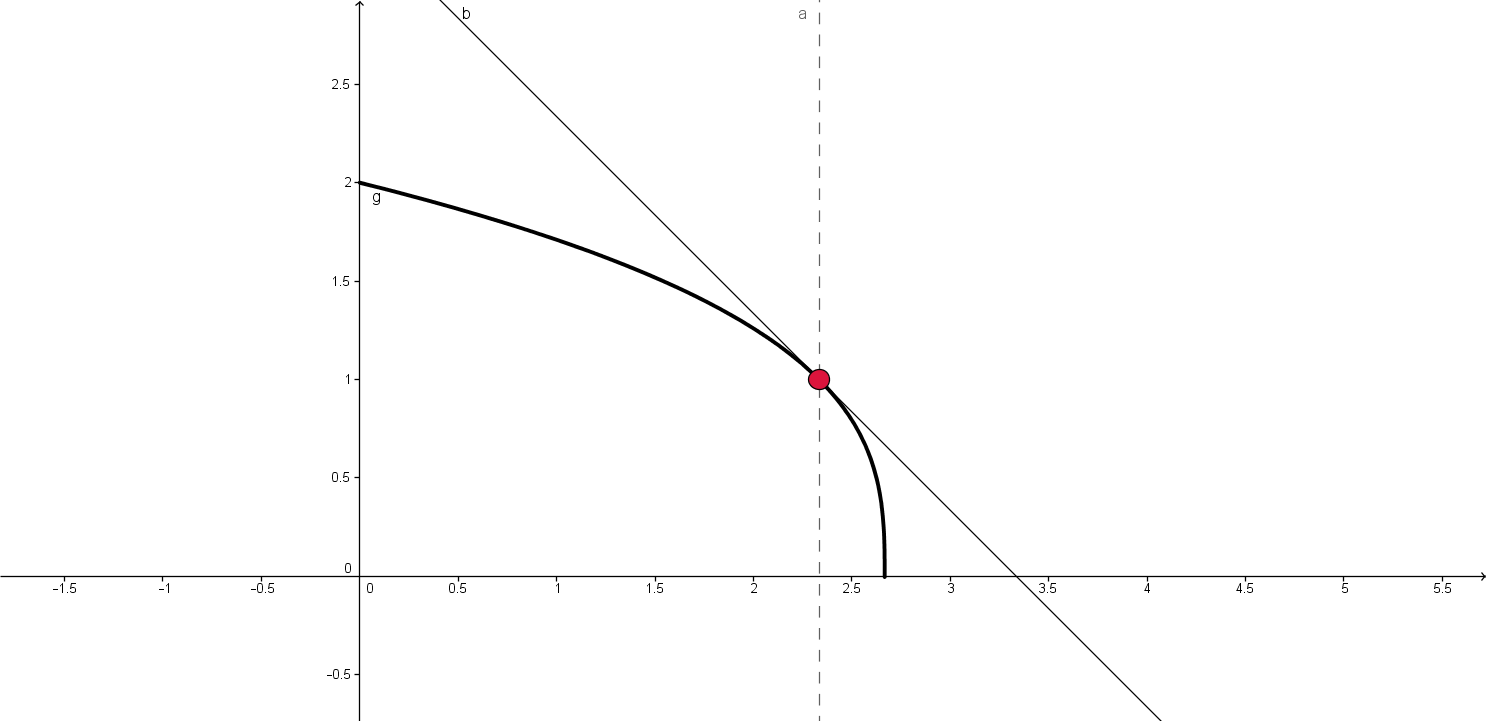
\includegraphics{img/volume.png}
	\end{center}
	
	Observe que a variação é negativa, confirmando a ideia de que o nível da água reduz quando ela vai esvaziando. E observando o gráfico podemos observar ainda que ele reduz mais rapidamente quanto menor o volume restante.
	\\
	
	\item Calcule a derivada $dy/dx$, onde:
	\begin{enumerate}
		\item $ y = \frac{x^5+x^3+1}{-x^4+x^2+3} $
		\begin{center}
			$ \left[ \frac{x^5+x^3+1}{-x^4+x^2+3} \right]' =$\\ $\frac{(5x^4+3x^2)(-x^4+x^2+3) - (-4x^3+2x)(x^5+x^3+1)}{(-x^4+x^2+3)^2} = $\\ $\frac{5x^4+3x^2}{-x^4+x^2+3} - \frac{(x^5+x^3+1)(-4x^3+2x)}{(-x^4+x^2+3)^2} = $\\
		\end{center}
		
		\item $ y = \tan(\sqrt{x^3+1}) $
		\begin{center}
			$ \left[ \tan(\sqrt{x^3+1}) \right]' = \frac{1}{cos^2(\sqrt{x^3+1})} \frac{(x^3+1)^{-\frac{1}{2}}}{2} $\\
			$ \left[ \tan(\sqrt{x^3+1}) \right]' = \frac{1}{2 cos^2(\sqrt{x^3+1}) \sqrt{x^3+1} } $
		\end{center}
		
		\item $ y = x^9 \cos^5(x) $
		\begin{center}
			$ \left[ x^9 \cos^5(x)\right]' = 9x^8 \cos^5(x) - 5x^9 \cos^4(x) \sin(x) $
		\end{center}
		
	\end{enumerate}
	
	\item Equacione a reta tangente á curva abaixo no ponto $(0,1)$:
	\begin{center}
		$ \left( x + y \right)^4 -7x^2 + y = 2  $\\
	\end{center}
	
	Podemos tomar $y$ em função de $x$, ou seja, $y(x)$ e queremos encontrar $y(x)'$.
	
	\begin{center}
		$ \left( x + y(x) \right)^4 -7x^2 + y(x) = 2  $\\
		$ 4\left( x + y(x) \right)^3(1+ y(x)') -14x + y(x)' = 0  $\\
		$ y(x)' = \frac{14x - 4(x+y)^3}{1 + 4(x+y)^3} $\\
	\end{center}
	
	Substituindo no ponto $(0,1)$, onde $y(x) = 1$, temos:
	\begin{center}
		$ y(x)' = -\frac{4}{5} $\\
	\end{center}
	Aplicando na equação da reta e considerando que passa pelo ponto $(0,1)$:
	\begin{center}
		$ y = -\frac{4}{5}x + 1 $\\
	\end{center}
	
	O problema está representado no gráfico abaixo:
	\begin{center}
		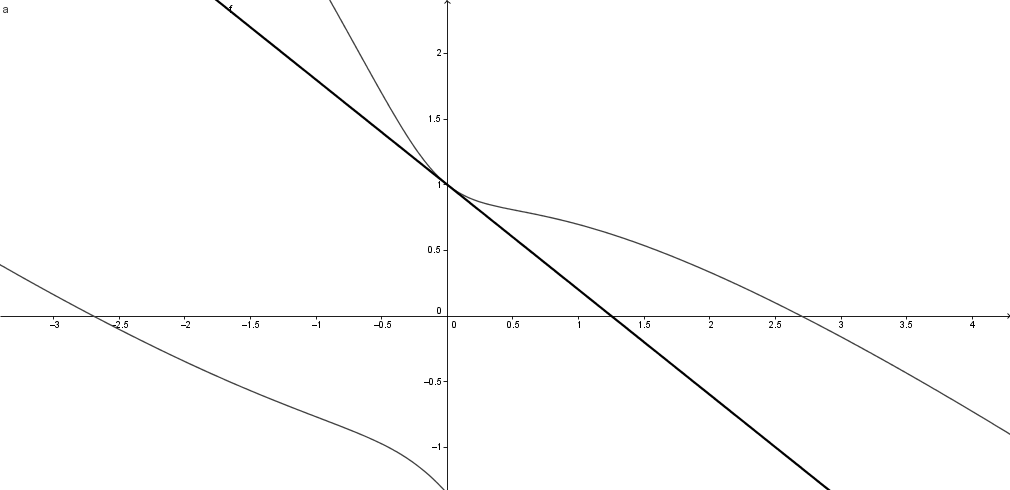
\includegraphics{img/reta.png}
	\end{center}
		
\end{enumerate}


\end{document}